\ifx\wholebook\relax \else
% ------------------------

\documentclass[b5paper]{ctexart}
\usepackage[nomarginpar
  %, margin=.5in
]{geometry}

\addtolength{\oddsidemargin}{-0.05in}
\addtolength{\evensidemargin}{-0.05in}
\addtolength{\textwidth}{0.1in}
\usepackage[cn]{../../../prelude}

\setcounter{page}{1}

\begin{document}

\title{二项式堆、斐波那契堆、配对堆}

\author{刘新宇
\thanks{{\bfseries 刘新宇 } \newline
  Email: liuxinyu95@gmail.com \newline}
  }

\maketitle
\fi

\markboth{二项式堆、斐波那契堆、配对堆}{基本算法}

\ifx\wholebook\relax
\chapter{二项式堆,斐波那契堆、配对堆}
\numberwithin{Exercise}{chapter}
\fi

\section{简介}
\label{introduction}

二叉堆使用二叉树存储元素,将二叉树扩展成$k$叉树\cite{K-ary-tree}($k>2$)甚至多棵树可得到更丰富的堆结构。本章介绍二项式堆,它由多棵$k$叉树的森林组成。如果延迟执行二项式堆的某些操作,就可以得到斐波那契堆。斐波那契堆将堆合并的性能从对数时间复杂度提升到常数时间,这对于图算法很重要。本章还介绍配对堆。它在实际中拥有最好的性能。

\section{二项式堆}
\label{sec:binomial-heap} \index{二项式堆}

二项式堆得名于牛顿二项式。它由一组$k$叉树的森林组成,每棵树的大小为二项式展开中的各项系数。牛顿证明了形如$(a + b)^n$的二项式展开后,各项系数可以表示为:

\be
(a + b)^n = a^n + \binom{n}{1} a^{n-1}b + ... + \binom{n}{n-1} a b^{n-1} + b
\ee

当$n$为自然数时,各项系数就呈现出帕斯卡三角形中的一行,如下图所示\footnote{中国称“贾宪”三角形。贾宪(1010-1070),牛顿在1665年证明了$n$为有理数时的情形,欧拉后来将$n$推广到实数。}\cite{wiki-pascal-triangle}。

\begin{verbatim}
    1
   1 1
  1 2 1
 1 3 3 1
1 4 6 4 1
...
\end{verbatim}

有多种方法可以产生一系列二项式系数,其中一种是使用递归。帕斯卡三角形中第一行为1,任何一行的两端为1,其它数字是上一行中左上和右上数字之和。

\subsection{二项式树}
\label{Binomial tree} \index{二项式树}

二项式树递归定义如下。一棵二项式树是一棵多叉树,并带有一个整数的秩(rank)。记秩为0的二项式树为$B_0$,秩为$n$的二项式树为$B_n$。

\begin{enumerate}
\item $B_0$树只包含一个节点;
\item $B_n$树由两棵$B_{n-1}$树组成,其中根节点元素较大的一棵是另一棵最左侧的子树。如图\ref{fig:link-bitree}所示。
\end{enumerate}

\begin{figure}[htbp]
  \centering
  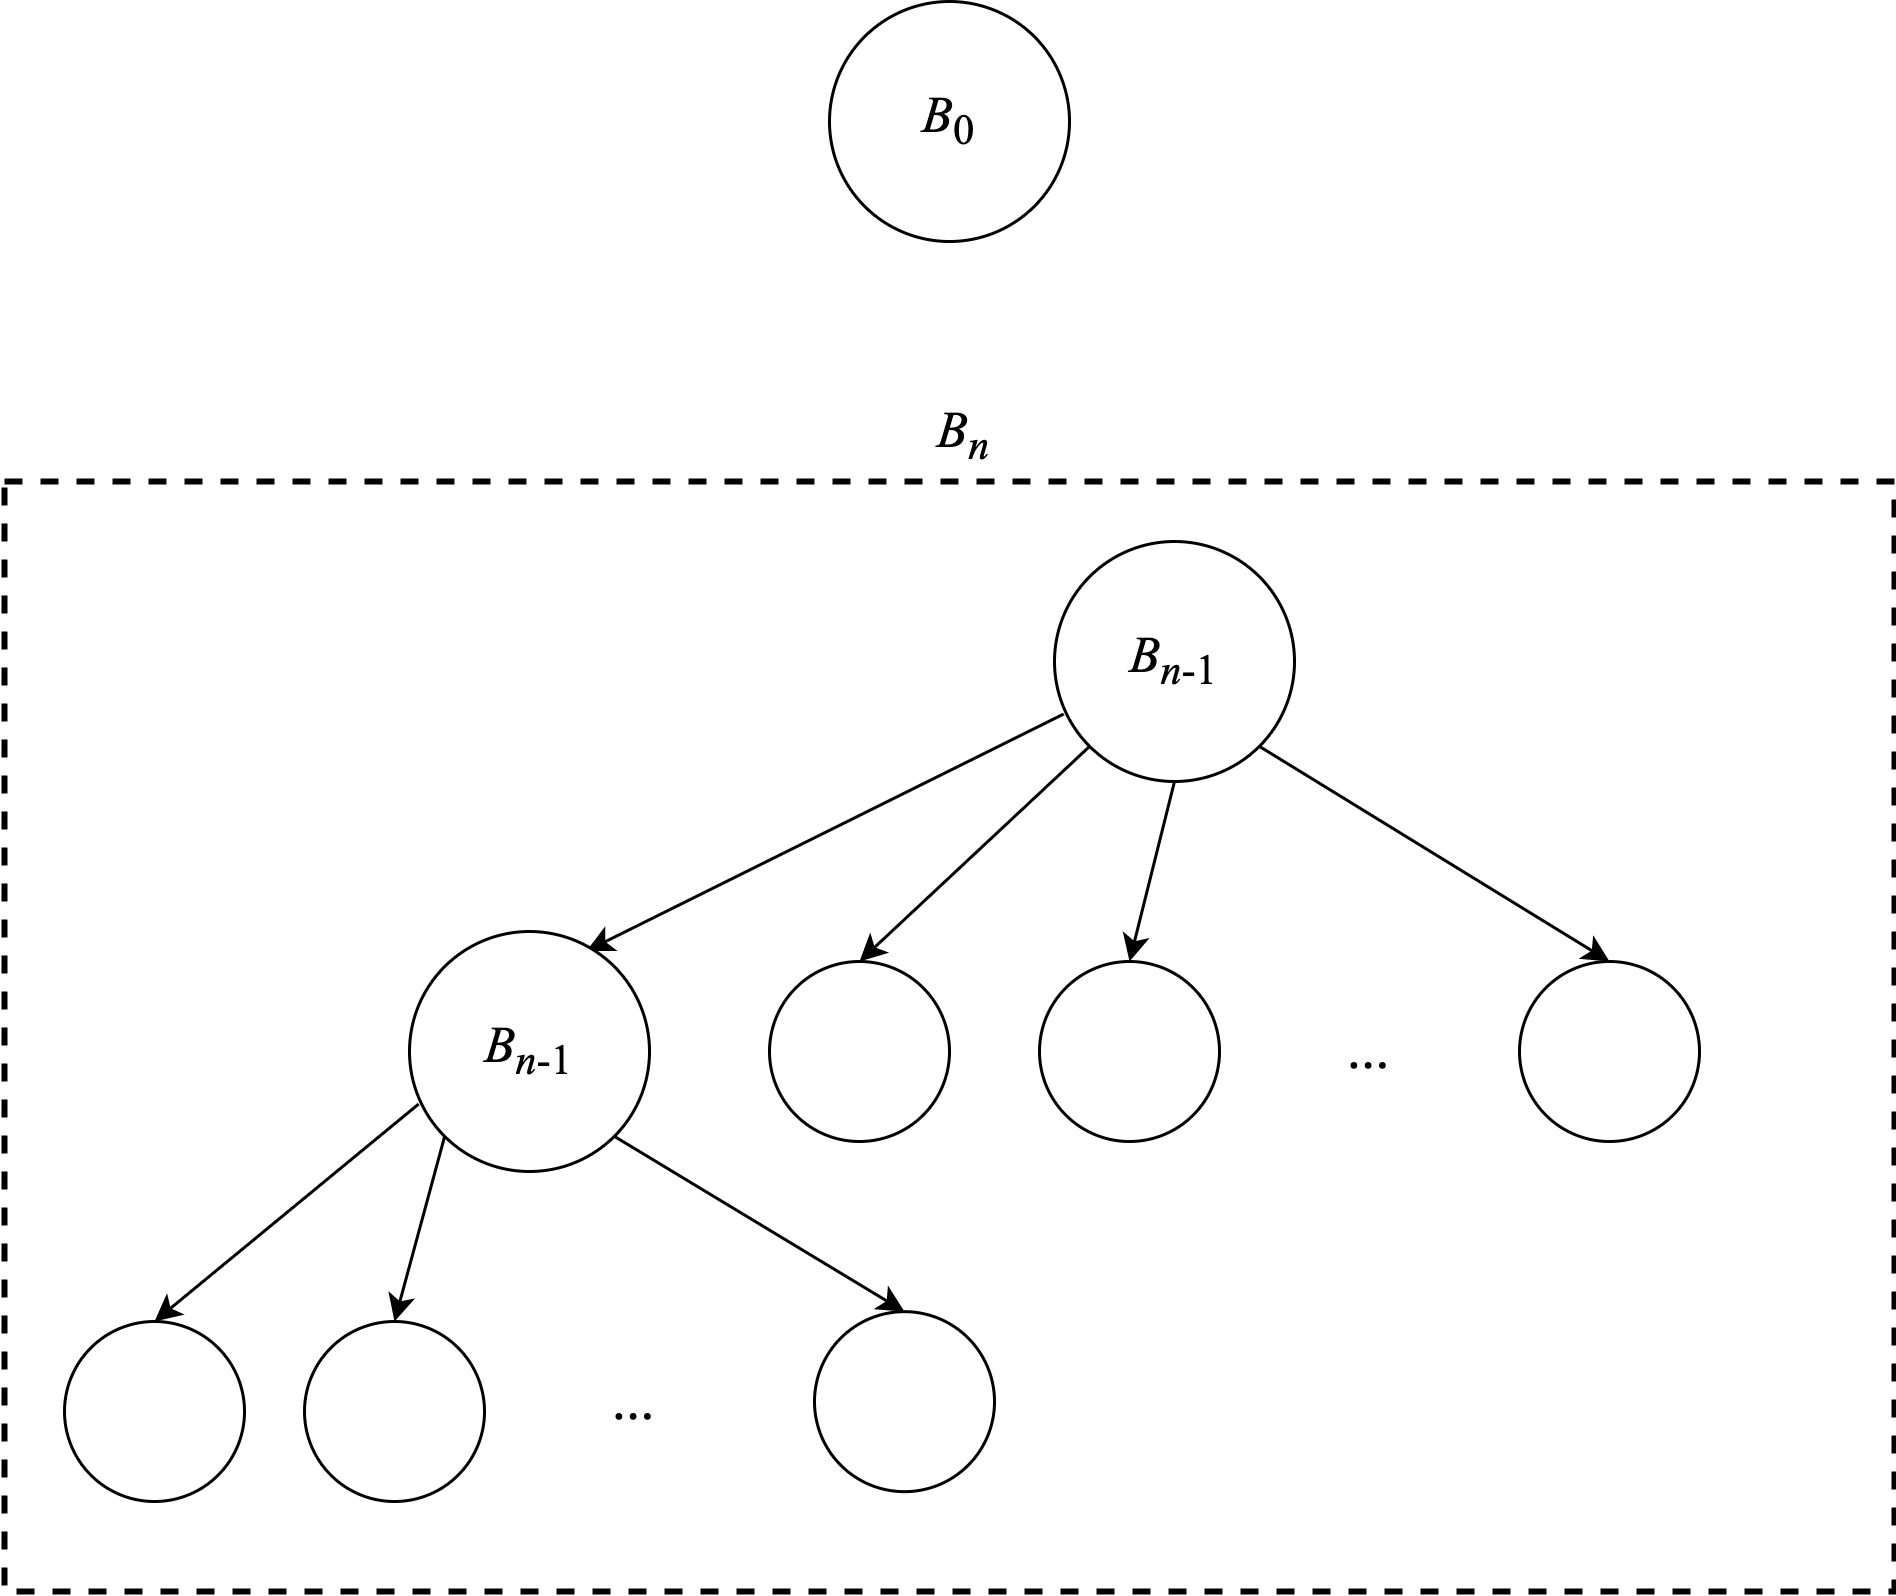
\includegraphics[scale=0.5]{img/btrees}
  \caption{二项式树}
  \label{fig:link-bitree}
\end{figure}

图\ref{fig:bitree-forms}给出了秩为0到4的二项式树例子:

\begin{figure}[htbp]
  \centering
  \subcaptionbox{$B_0$}{\hspace{0.05\textwidth}\includegraphics[scale=0.5]{img/b0tree}\hspace{0.05\textwidth}}
  \subcaptionbox{$B_1$}{\hspace{0.05\textwidth}\includegraphics[scale=0.5]{img/b1tree}\hspace{0.05\textwidth}}
  \subcaptionbox{$B_2$}{\includegraphics[scale=0.5]{img/b2tree}}
  \subcaptionbox{$B_3$}{\includegraphics[scale=0.5]{img/b3tree}} \\
  \subcaptionbox{$B_4$}{\includegraphics[scale=0.5]{img/b4tree}……}
  \caption{秩为0、1、2、3、4……的二项式树}
  \label{fig:bitree-forms}
\end{figure}

观察这些二项式树,可以发现$B_n$中每行的节点数目恰好是二项式系数。例如$B_4$第0层有1个节点(根节点),第1层有4个节点,第2层有6个节点,第3层有4个节点,第4层有1个节点。它们恰好是帕斯卡三角形的第4行(从第0行开始):1、4、6、4、1。这就是二项式树名字的由来。进一步我们可以得知二项式树$B_n$中含有$2^n$个元素。

\index{二项式堆!定义}
一个二项式堆包含一组二项式树(二项式树森林),它满足如下性质:

\begin{enumerate}
\item 每棵树都满足\textbf{堆性质},对于小顶堆,任意节点元素都不小于($\geq$)父节点元素;
\item 堆中任何两棵二项式树的秩都不同。
\end{enumerate}

从性质2可以导出一个结果:含有$n$个元素的二项式堆,如果将$n$转换为二进制数$(a_m ... a_1 a_0)_2$,其中$a_0$是最低位(LSB),$a_m$是最高位(MSB),若$a_i=0$,则堆中不存在秩为$i$的二项式树,若$a_i = 1$,则堆中一定含有一棵秩为$i$的树。例如,设二项式堆含有5个元素,5的二进制为101,堆中含有两棵二项式树,一棵秩为0、一棵秩为2。图\ref{fig:bheap2}中的二项式堆含有19个元素,$19 = (10011)_2$,含有一棵$B_0$树、一棵$B_1$树、一棵$B_4$树。

\begin{figure}[htbp]
  \centering
  \includegraphics[scale=0.5]{img/bheap2}
  \caption{含有19个元素的二项式堆}
  \label{fig:bheap2}
\end{figure}

我们将二项式树定义为多叉树,带有一个根节点元素$k$、秩$r$、和若干子树$ts$,记为$(r, k, ts)$。定义二项式堆为按照秩递增的二项式树的列表:

\lstset{frame=single}
\begin{Haskell}
data BiTree a = Node Int a [BiTree a]

type BiHeap a = [BiTree a]
\end{Haskell}

\index{左侧孩子,右侧兄弟}
有一种叫做“左侧孩子,右侧兄弟”\cite{CLRS}的方法,可以复用二叉树的结构来定义$k$叉树。每个节点包含左侧和右侧部分:左侧部分指向节点的第一棵子树,右侧部分指向兄弟节点。所有兄弟节点组成一个链表,如图\ref{fig:lcrs}所示。也可以直接利用数组或列表来表示一个节点的子树。

\begin{figure}[htbp]
  \centering
  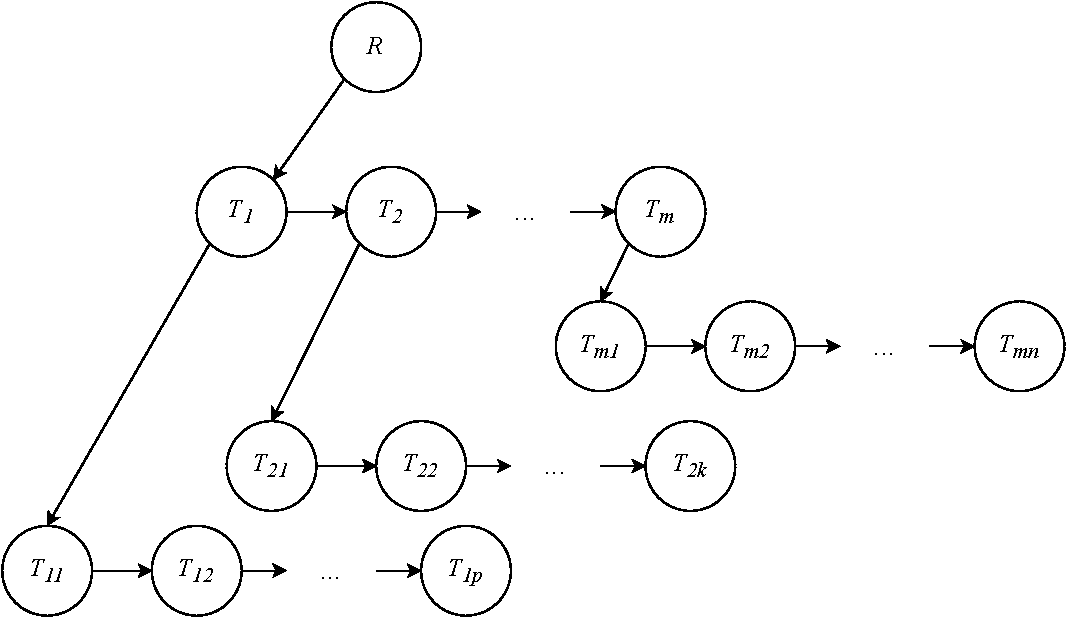
\includegraphics[scale=0.5]{img/left-child-right-sibling}
  \caption{$R$为根节点,$T_1, T_2, ..., T_m$为$R$的子树。$R$的左侧为$T_1$,右侧为空。$T_{11}, ..., T_{1p}$为$T_1$的子树。$T_1$的左侧是子树$T_{11}$,右侧是兄弟节点$T_2$。$T_2$的左侧是子树$T_{21}$,右侧是兄弟节点。}
  \label{fig:lcrs}
\end{figure}

\subsection{树的链接}
\index{二项式堆!链接}

我们定义链接操作从两棵二项式树$B_n$构造出$B_{n+1}$。比较两棵树的根节点元素,选择较小的作为新的根,然后将另一棵置于其它子树前面,如图\ref{fig:link-xy}所示。

\be
link\ (r, x, ts)\ (r, y, ts') = \begin{cases}
  x < y: & (r + 1, x, (r, t, ts') : ts) \\
  \text{否则}: & (r + 1, y, (r, x, ts): ts') \\
  \end{cases}
\label{eq:link}
\ee

\begin{figure}[htbp]
  \centering
  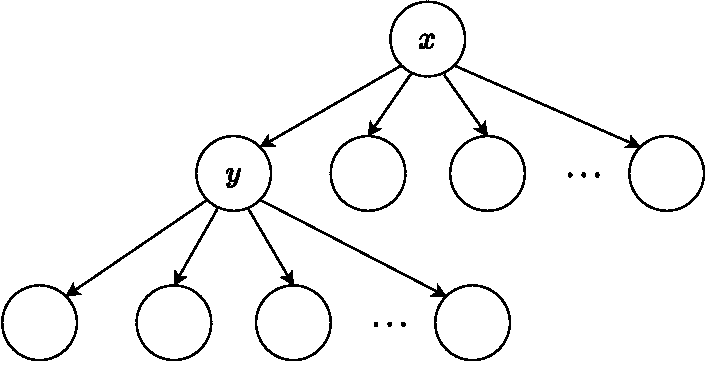
\includegraphics[scale=0.5]{img/link-bitree-xy}
  \caption{如果$x < y$,将$y$作为$x$的第一棵子树。}
  \label{fig:link-xy}
\end{figure}

使用“左侧孩子,右侧兄弟”的实现如下。如图\ref{fig:link-lcrs}所示。链接操作可以在常数时间内完成。

\begin{algorithmic}[1]
\Function{Link}{$x, y$}
  \If{\Call{Key}{$y$} $<$ \Call{Key}{$x$}}
    \State Exchange $x \leftrightarrow y$
  \EndIf
  \State \Call{Sibling}{$y$} $\gets$ \Call{Sub-Trees}{$T_1$}
  \State \Call{Sub-Trees}{$x$} $\gets y$
  \State \Call{Parent}{$y$} $\gets x$
  \State \Call{Rank}{$x$} $\gets$ \Call{Rank}{$y$} + 1
  \State \Return $x$
\EndFunction
\end{algorithmic}

\begin{Exercise}
\Question{编程产生帕斯卡三角形}
\Question{证明二项式树$B_n$中第$i$行的节点数为$\binom{n}{i}$。}
\Question{证明二项式树$B_n$中含有$2^n$个节点。}
\Question{用容器保存子树,实现二项式树的链接。这种方式有何问题,怎样解决?}
\end{Exercise}

\begin{Answer}
\Question{编程产生帕斯卡三角形
\begin{Haskell}[frame=single]
pascal = gen [1] where
  gen cs (x:y:xs) = gen ((x + y) : cs) (y:xs)
  gen cs _ = 1 : cs
\end{Haskell}
}
\Question{证明二项式树$B_n$中第$i$行的节点数为$\binom{n}{i}$。
\begin{proof}
使用数学归纳法。$B_0$只有一个根节点。设$B_n$中每行满足二项式系数。树$B_{n+1}$由两棵$B_n$组成。第0行为根节点:$1 = \binom{n+1}{0}$。第$i$行的节点包含两部分,一部分是最左侧子树$B_n$的第$i-1$行,一部分是另一棵$B_n$的第$i$行,总共有:

\[
\begin{array}{rcl}
\binom{n}{i-1} + \binom{n}{i} & = & \dfrac{n!}{(i-1)!(n-i+1)!} + \dfrac{n!}{i!(n-i)!} \\
 & = & \dfrac{n!}{(i-1)!(n-i)!}(\dfrac{1}{i} - \dfrac{1}{n-i+1}) \\
 & = & \dfrac{n!}{(i-1)!(n-i)!}\dfrac{n+1}{i(n-i+1)} \\
 & = & \dfrac{(n+1)!}{i!(n-i+1)!} \\
 & = & \binom{n+1}{i} \\
\end{array}
\]
\end{proof}
}
\Question{证明二项式树$B_n$中含有$2^n$个节点。
\begin{proof}
根据上一练习中证明的结果,$B_n$中各行节点相加为:
\[
\begin{array}{cll}
  & \binom{n}{0} + \binom{n}{1} + ... + \binom{n}{n} & \text{各行相加} \\
= & (1 + 1)^n & \text{令二项式} (a + b)^n \text{中}a = b = 1 \\
= & 2^n & \\
\end{array}
\]
\end{proof}
}
\Question{用容器保存子树,实现二项式树的链接程序。这种方式有何问题,怎样解决?

如果用数组保存子树,在所有元素前插入需要线性时间:

\begin{algorithmic}[1]
\Function{Link'}{$T_1, T_2$}
  \If{\Call{Key}{$T_2$} $<$ \Call{Key}{$T_1$}}
    \State Exchange $T_1 \leftrightarrow T_2$
  \EndIf
  \State \Call{Parent}{$T_2$} $\gets T_1$
  \State \textproc{Insert}(\Call{Sub-Trees}{$T_1$}, 1, $T_2$)
  \State \Call{Rank}{$T_1$} $\gets$ \Call{Rank}{$T_2$} + 1
  \State \Return $T_1$
\EndFunction
\end{algorithmic}

为此,我们可以将子树逆序保存。这样将新树附加到末尾只需要常数时间。
}
\end{Answer}

\subsection{插入}
\index{二项式堆!插入} \index{二项式堆!push}

我们令堆中二项式树按照秩递增排列,并在插入新树时保持秩的顺序:

\be
\begin{array}{rcl}
ins\ t\ [\ ] & = & [t] \\
ins\ t\ (t':ts) & = & \begin{cases}
  rank\ t < rank\ t': & t:t':ts \\
  rank\ t' < rank\ t: & t' : ins\ t\ ts \\
  \text{否则}: & ins\ (link\ t\ t')\ ts  \\
\end{cases}
\end{array}
\ee

其中$rank\ (r, k, ts) = r$,获取一棵二项式树的秩。如果堆为空$[\ ]$,则新树$t$成为堆中唯一的树;否则,我们比较$t$和堆中第一棵树$t'$的秩。如果$t$的秩较小,则$t$成为第一棵树;如果$t'$的秩较小,我们递归地将$t$插入到剩余的树中;如果秩相等,就将$t$、$t'$链接成一棵更大的树,然后递归地插入到剩余的树中。如果有$n$个元素,堆中最多有$O(\lg n)$棵二项式树。$ins$最多执行$O(\lg n)$次常数时间的链接。其时间复杂度为$O(\lg n)$\footnote{这一过程和两个二进制数的加法相似,可以引出一类问题:数值表示(numeric representation)\cite{okasaki-book}。}。使用$ins$,我们可以定义二项式堆的插入算法。先将待插入元素$x$放入一棵只有一个叶子节点树中,然后再插入到堆中:

\be
insert\ x = ins\ (0, x, [\ ])
\ee

这一定义是克里化的。我们可以利用叠加操作将若干元素插入到堆中:

\be
\textit{fromList} = foldr\ insert\ [\ ]
\ee

对应的“左侧孩子,右侧兄弟”实现如下:\label{alg:insert-tree}

\begin{algorithmic}[1]
\Function{Insert-Tree}{$T, H$}
  \State $\perp \gets p \gets$ \Call{Node}{$0$, NIL, NIL}
  \While{$H \neq$ NIL 且 \Call{Rank}{$H$} $\leq$ \Call{Rank}{$T$}}
    \State $T_1 \gets H$
    \State $H \gets $ \Call{Sibling}{$H$}
    \If{\Call{Rank}{$T$} = \Call{Rank}{$T_1$}}
      \State $T \gets$ \Call{Link}{$T, T_1$}
    \Else
      \State \Call{Sibling}{$p$} $\gets T_1$
      \State $p \gets T_1$
    \EndIf
  \EndWhile
  \State \Call{Sibling}{$p$} $\gets T$
  \State \Call{Sibling}{$T$} $\gets H$
  \State \Return \Call{Remove-First}{$\perp$}
\EndFunction
\Statex
\Function{Remove-First}{$H$}
  \State $n \gets$ \Call{Sibling}{$H$}
  \State \Call{Sibling}{$H$} $\gets$ NIL
  \State \Return $n$
\EndFunction
\end{algorithmic}

\subsection{堆合并}
\index{二项式树!合并}

合并两个二项式堆相当于合并两个二项式树森林。合并结果中没有秩相同的树,并且按照秩递增。合并过程和归并排序类似。每次从两个堆中各取出第一棵树,比较它们的秩,将较小的一棵放入结果中。如果两棵树的秩相等,我们将它们链接成为一棵较大的树,然后递归插入到合并结果中。

\be
\begin{array}{rcl}
merge\ ts_1\ [\ ] & = & ts_1 \\
merge\ [\ ]\ ts_2 & = & ts_2 \\
merge\ (t_1:ts_1)\ (t_2:ts_2) & = & \begin{cases}
  rank\ t_1 < rank\ t_2: & t_1 : (merge\ ts_1\ (t_2:ts_2)) \\
  rank\ t_2 < rank\ t_1: & t_2 : (merge\ (t_1:ts_1)\ ts_2) \\
  \text{否则}: & ins\ (link\ t_1\ t_2)\ (merge\ ts_1\ ts_2) \\
  \end{cases}
\end{array}
\ee

当$t_1$、$t_2$秩相同时,我们也可以将链接后的树插入回任意一个堆,然后递归合并:

\[
merge\ (ins\ (link\ t_1\ t_2)\ ts_1)\ ts_2
\]

用这种方式可以消除递归,用迭代的方式实现堆合并:

\begin{algorithmic}[1]
\Function{Merge}{$H_1, H_2$}
  \State $H \gets p \gets$ \Call{Node}{0, NIL, NIL}
  \While{$H_1 \neq$ NIL 且 $H_2 \neq$ NIL}
    \If{\Call{Rank}{$H_1$} $<$ \Call{Rank}{$H_2$}}
      \State \Call{Sibling}{$p$} $\gets H_1$
      \State $p \gets$ \Call{Sibling}{$p$}
      \State $H_1 \gets$ \Call{Sibling}{$H_1$}
    \ElsIf{\Call{Rank}{$H_2$} $<$ \Call{Rank}{$H_1$}}
      \State \Call{Sibling}{$p$} $\gets H_2$
      \State $p \gets$ \Call{Sibling}{$p$}
      \State $H_2 \gets$ \Call{Sibling}{$H_2$}
    \Else \Comment{秩相等}
      \State $T_1 \gets H_1, T_2 \gets H_2$
      \State $H_1 \gets$ \Call{Sibling}{$H_1$}, $H_2 \gets$ \Call{Sibling}{$H_2$}
      \State $H_1 \gets $ \textproc{Insert-Tree}(\Call{Link}{$T_1, T_2$}, $H_1$)
    \EndIf
  \EndWhile
  \If{$H_1 \neq$ NIL}
    \State \Call{Sibling}{$p$} $\gets H_1$
  \EndIf
  \If{$H_2 \neq$ NIL}
    \State \Call{Sibling}{$p$} $\gets H_2$
  \EndIf
  \State \Return \Call{Remove-First}{$H$}
\EndFunction
\end{algorithmic}

设堆$H_1$中有$m_1$棵树,堆$H_2$中有$m_2$棵树。合并后的结果中最多有$m_1 + m_2$棵树。如果没有秩相同的树,则合并时间为$O(m_1 + m_2)$。如果存在秩相同的树,最多需要调用$O(m_1 + m_2)$次$ins$。考虑$m_1 = 1 + \lfloor \lg n_1 \rfloor$,$m_2 = 1 + \lfloor \lg n_2 \rfloor$,其中$n_1$和$n_2$是两个堆各自的元素数,且$\lfloor \lg n_1 \rfloor + \lfloor \lg n_2 \rfloor \leq 2 \lfloor \lg n \rfloor$,其中$n = n_1 + n_2$。最终合并的复杂度为$O(\lg n)$。

\subsection{弹出}
\index{二项式堆!弹出}

二项式堆中,每棵树的根节点保存了树中的最小元素。但根节点元素间的大小关系是任意的。为了获取堆中的最小元素,需要在全部根节点中查找。因为堆中有$\lg n$棵树,所以获取最小值的时间复杂度为$O(\lg n)$。但是弹出操作不仅找出最小元素,还需要将其删除并保持堆性质。设堆中的二项式树为$B_i, B_j, ..., B_p, ..., B_m$。设$B_p$的根节点为堆中最小元素。将其删除后会产生$p$棵子二项式树,秩为$p-1, p-2, ..., 0$。我们可以将$p$棵子树逆序,形成一个新二项式堆$H_p$。除去$B_p$的树也构成一个二项式堆$H' = H - [B_p]$。将$H_p$和$H'$合并就可以得到最终结果,如图\ref{fig:bheap-del-min}所示。我们首先定义从堆中寻找最小元素的操作:

\begin{figure}[htbp]
  \centering
  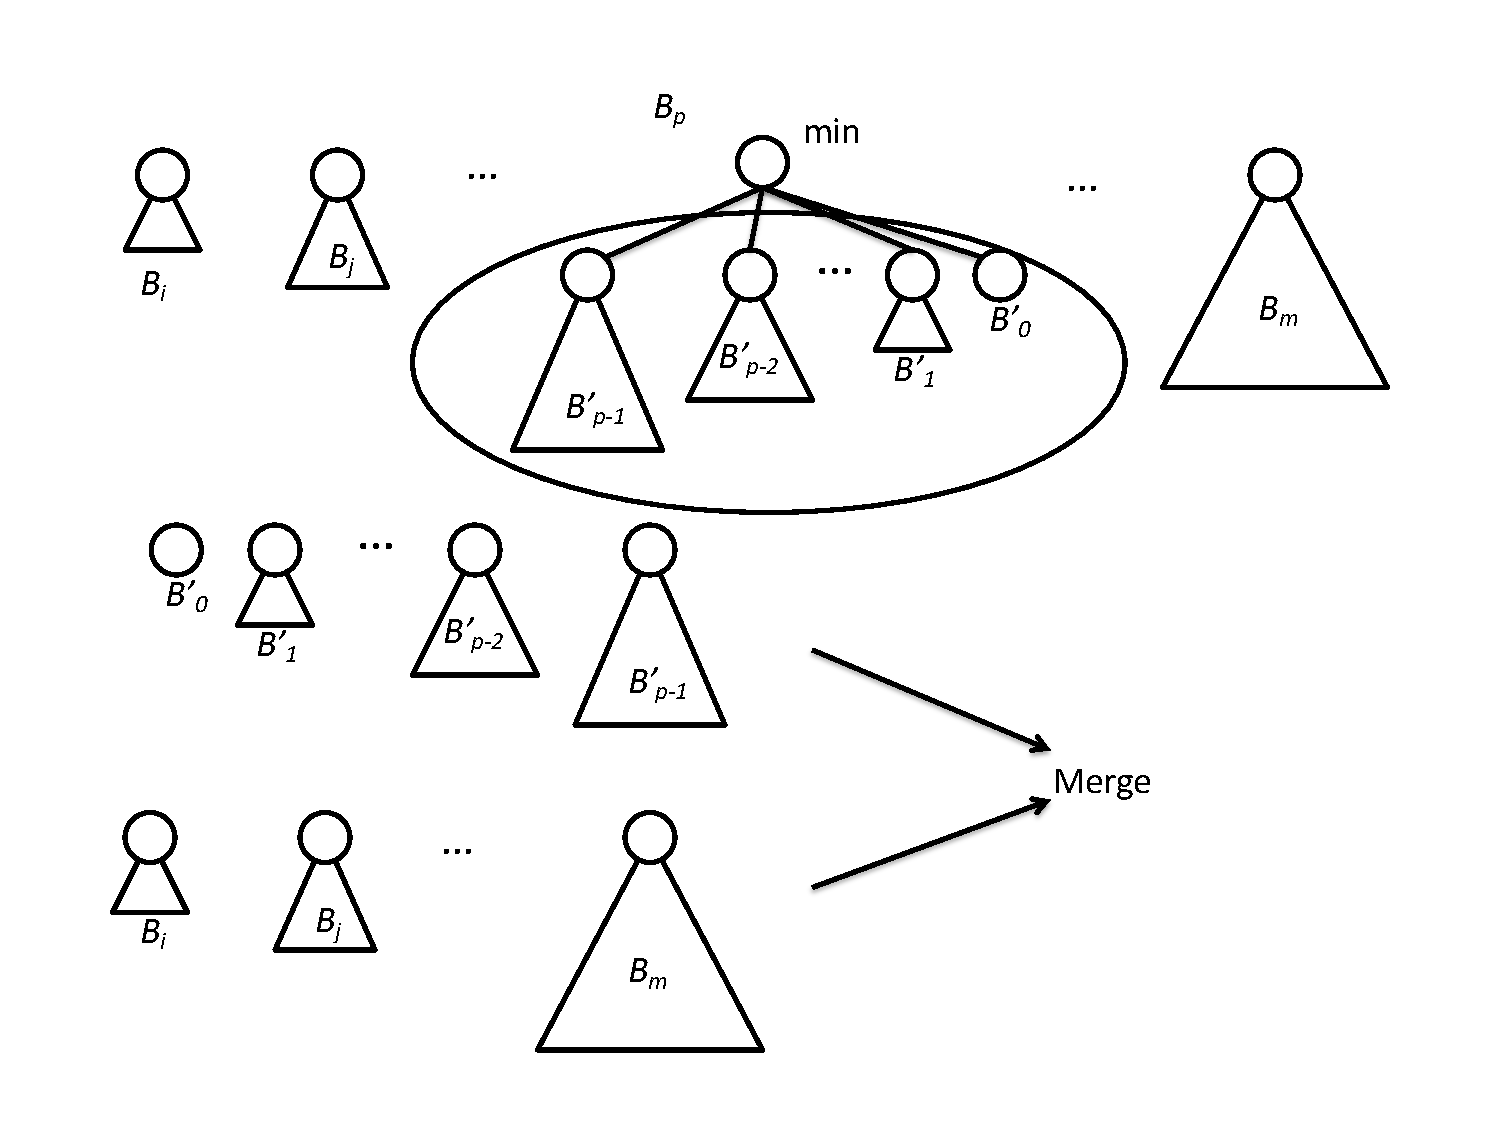
\includegraphics[scale=0.4]{img/bheap-pop}
  \caption{二项式堆的弹出操作}
  \label{fig:bheap-del-min}
\end{figure}

\be
top\ (t:ts) = foldr\ f\ (key\ t)\ ts
\ee

其中

\[
f\ (r, x, ts)\ y = min\ x\ y
\]

这相当于遍历堆中的所有树,找出根节中存储的最小值:

\begin{algorithmic}[1]
\Function{Top}{$H$}
  \State $m \gets \infty$
  \While{$H \neq$ NIL}
    \State $m \gets$ \textproc{Min}($m$, \Call{Key}{$H$})
    \State $H \gets $ \Call{Sibling}{$H$}
  \EndWhile
  \State \Return $m$
\EndFunction
\end{algorithmic}

为了实现弹出,我们需要从堆中分离出最小元素所在的树:

\be
\begin{array}{rcl}
min'\ [t] & = & (t, [\ ]) \\
min'\ (t:ts) & = & \begin{cases}
  key\ t < key\ t': & (t, ts), \text{其中}: (t', ts') = min'\ ts \\
  \text{否则}: & (t', t:ts')
  \end{cases}
\end{array}
\ee

其中$key\ (r, k, ts) = k$获取二项式树中的根节点元素。$min'$的结果为一对值:最小元素所在的树,和其它的树。接下来就可以定义弹出操作:

\be
pop\ H = (k, merge\ (reverse\ ts)\ H'), \text{其中}: ((r, k, ts), H') = min'\ H
\ee

对应的迭代实现为:

\begin{algorithmic}[1]
\Function{Pop}{$H$}
  \State $(T_m, H) \gets$ \Call{Extract-Min}{$H$}
  \State $H \gets$ \textproc{Merge}($H$, \textproc{Reverse}(\Call{Sub-Trees}{$T_m$}))
  \State \Call{Sub-Trees}{$T_m$}
  \State \Return (\Call{Key}{$T_m$}, $H$)
\EndFunction
\end{algorithmic}

其中反转操作的实现见第一章,\textproc{Extract-Min}的迭代实现如下:

\begin{algorithmic}[1]
\Function{Extract-Min}{$H$}
  \State $H' \gets H, p \gets$ NIL
  \State $T_m \gets T_p \gets$ NIL
  \While{$H \neq$ NIL}
    \If{$T_m =$ NIL 或 \Call{Key}{$H$} $<$ \Call{Key}{$T_m$}}
      \State $T_m \gets H$
      \State $T_p \gets p$
    \EndIf
    \State $p \gets H$
    \State $H \gets $ \Call{Sibling}{$H$}
  \EndWhile
  \If{$T_p \neq$ NIL}
    \State \Call{Sibling}{$T_p$} $\gets$ \Call{Sibling}{$T_m$}
  \Else
    \State $H' \gets$ \Call{Sibling}{$T_m$}
  \EndIf
  \State \Call{Sibling}{$T_m$} $\gets$ NIL
  \State \Return $(T_m, H')$
\EndFunction
\end{algorithmic}

使用弹出操作可以实现堆排序。首先从待排序元素构建一个二项式堆,然后不断从中弹出最小元素。

\be
sort  = heapSort \circ fromList
\ee

其中$heapSort$实现如下:

\be
\begin{array}{rcl}
  heapSort\ [\ ] & = & [\ ] \\
  heapSort\ H & = & k : (heapSort\ H'), \text{其中}: (k, H') = pop\ H
\end{array}
\ee

二项式堆的插入、合并的时间复杂度在最坏情况下是$O(\lg n)$。他们的分摊复杂度为常数时间,我们这里略去了分摊复杂度的证明。

\section{斐波那契堆}
\label{fib-heap} \index{斐波那契堆}

“斐波那契堆”的命名很有趣,实际上斐波那契堆的结构和斐波那契数列无关。斐波那契堆的作者Michael L. Fredman和Robert E. Tarjan在证明这种堆的时间性能时使用了斐波那契数列的性质,于是他们决定给这种堆命名为“斐波那契堆”\cite{CLRS}。

% ================================================================
%                 Definition
% ================================================================
\subsection{定义}

斐波那契堆本质上是一个惰性二项式堆。但是这并不意味着二项式堆在支持惰性求值的环境下(例如Haskell)自动就成为斐波那契堆。惰性环境仅仅对于实现提供了便利。例如\cite{hackage-fibq}中给出了一个简洁的实现。

斐波那契堆在理论上具有良好的性能。除弹出之外所有的操作分摊性能都达到了常数时间$O(1)$。本节中,我们给出的实现和常见的实现\cite{CLRS}有所不同。主要思想来自于Okasaki的工作\cite{okasaki-fibh}。

首先我们对比一下二项式堆和斐波那契堆的性能(确切的说,是我们希望斐波那契堆达到的性能目标)。

\begin{table}[htbp]
\centering
\begin{tabular}{l | c | r}
  \hline
  操作 & 二项式堆 & 斐波那契堆 \\
  \hline
  插入 & $O(\lg n)$ & $O(1)$ \\
  合并 & $O(\lg n)$ & $O(1)$ \\
  top & $O(\lg n)$ & $O(1)$ \\
  弹出 & $O(\lg n)$ & 分摊 $O(\lg n)$ \\
  \hline
\end{tabular}
\caption{斐波那契堆的性能目标}
\end{table}

在二项式堆中,插入一个新元素时,哪里是瓶颈呢?新元素$x$被放入只有一个叶子节点的树中,然后这棵树被插入到森林中。

在此期间,树按照Rank的单调递增顺序插入,如果Rank相等,则进行链接,然后再递归,因此性能为$O(\lg n)$。

使用惰性策略,我们可以将按照Rank的顺序插入和链接等操作推迟进行。仅仅将只有一个叶子节点的树放入森林中。这样带来的问题是,当获取最小元素时,性能会变得很差。这是因为我们需要检查森林中的所有树,而树的总数不只是$O(\lg n)$。

为了在常数时间获得堆顶元素,我们需要记录哪一棵树的根节点保存了最小元素。

根据这一思路,我们可以在二项式堆的基础上给出斐波那契堆定义。如下面的Haskell例子程序所示,我们复用二项式树的定义:

\lstset{language=Haskell}
\begin{lstlisting}[style=Haskell]
data BiTree a = Node { rank :: Int
                     , root :: a
                     , children :: [BiTree a]}
\end{lstlisting}

斐波那契堆要么为空,要么是一个二项式树的森林,其中含有最小元素的树被单独保存。

\begin{lstlisting}[style=Haskell]
data FibHeap a = E | FH { size :: Int
                        , minTree :: BiTree a
                        , trees :: [BiTree a]}
\end{lstlisting}

方便起见,我们将堆中元素的个数也记录下来。

斐波那契堆也可以用命令式的方式定义,如下面的C语言例子代码。

\lstset{language=C}
\begin{lstlisting}
struct node {
    Key key;
    struct node *next, *prev, *parent, *children;
    int degree; //即Rank

    int mark;
};

struct FibHeap {
    struct node *roots;
    struct node *minTr;
    int n; //节点的个数
};
\end{lstlisting}

上面的代码中,Key可以是任何可比较大小的类型,简单起见我们假设类型为整数。

\lstset{language=C}
\begin{lstlisting}
typedef int Key;
\end{lstlisting}

我们在命令式实现中,使用循环双向链表\cite{CLRS}。这样可以简化很多操作并提供快速的性能。我们增加了两个额外的字段。一个是\texttt{degree}(即Rank),定义为一个节点中子树的数目;标志$mark$仅用于减小元素值的操作。我们稍后会对$mark$的作用加以介绍。


% ================================================================
%          Basic Heap operations
% ================================================================
\subsection{基本堆操作}

由于斐波那契堆本质上是惰性的二项式堆,我们将复用很多二项式堆的算法。

\subsubsection{插入新元素}
\index{斐波那契堆!插入}

可以认为二项式堆的插入算法是一种特殊的合并操作,其中一个堆仅含有一棵一个叶节点的树。

\be
insert(H, x) = merge(H, singleton(x))
\label{eq:fib-insert}
\ee

其中$singleton$是一个辅助函数,它构建出仅含有一个元素的树。

\[
singleton(x) = FibHeap(1, node(1, x, \phi), \phi)
\]

函数$FibHeap()$接受3个参数,一个是大小(size),因为只有一个元素,所以值为1,一棵特殊的树,树根存有堆中的最小元素,以及森林中剩余二项式树的列表。函数$node()$和以前的含意一样,它从一个Rank值,一个元素,和一组子树列表构建一棵二项式树。

插入操作也可以实现为向森林中追加一个新节点,然后更新存有最小元素的树。

\begin{algorithmic}[1]
\Function{Insert}{$H, k$}
  \State $x \gets$ \Call{Singleton}{$k$} \Comment{将$x$装入一节点}
  \State append $x$ to root list of $H$
  \If{$T_{min}(H) = NIL \lor k <$ \Call{Key}{$T_{min}(H)$} }
    \State $T_{min}(H) \gets x$
  \EndIf
  \State \Call{n}{$H$} $\gets$ \Call{n}{$H$}+1
\EndFunction
\end{algorithmic}

其中函数$T_{min}()$返回存有最小元素的树。

下面的C语言例子代码实现了这一插入算法。

\lstset{language=C}
\begin{lstlisting}
struct FibHeap* insert_node(struct FibHeap* h, struct node* x) {
    h = add_tree(h, x);
    if(h->minTr == NULL || x->key < h->minTr->key)
        h->minTr = x;
    h->n++;
    return h;
}
\end{lstlisting}

\begin{Exercise}
选择一门命令式编程语言,实现完整的插入算法。这也是循环双向链表操作的一道习题。
\end{Exercise}

\subsubsection{堆合并}
\index{斐波那契堆!合并}

和二项式堆不同,我们在合并时并不立即进行链接操作,而是推迟到以后。这样仅仅将两个堆中的树放到一起,然后选出新的含有最小元素的树记录下来。

\be
merge(H_1, H_2) = \left \{
  \begin{array}
  {r@{\quad:\quad}l}
  H_1 & H_2 = \phi \\
  H_2 & H_1 = \phi \\
  FibHeap(s_1 + s_2, {T_1}_{min}, \{ {T_2}_{min} \} \cup \mathbb{T}_1 \cup \mathbb{T}_2) & root({T_1}_{min}) < root({T_2}_{min}) \\
  FibHeap(s_1 + s_2, {T_2}_{min}, \{ {T_1}_{min} \} \cup \mathbb{T}_1 \cup \mathbb{T}_2) & otherwise \\
  \end{array}
\right .
\ee

其中$s_1$和$s_2$分别时两个堆$H_1$和$H_2$的大小;${T_1}_{min}$和${T_2}_{min}$分别是两个堆中存有最小的元素的树。$\mathbb{T}_1 = \{{T_1}_1, {T_1}_2, ...\}$是堆$H_1$的森林中其余的树;而$\mathbb{T}_2$的含意类似,它包含堆$H_2$中森林里剩余的树。函数$root(T)$返回一棵二项式树的根节点元素。

只要$\cup$操作的性能为常数时间,合并算法的性能就是常数时间。下面的Haskell例子程序实现了合并操作。

\lstset{language=Haskell}
\begin{lstlisting}[style=Haskell]
merge h E = h
merge E h = h
merge h1@(FH sz1 minTr1 ts1) h2@(FH sz2 minTr2 ts2)
    | root minTr1 < root minTr2 = FH (sz1+sz2) minTr1 (minTr2:ts2++ts1)
    | otherwise = FH (sz1+sz2) minTr2 (minTr1:ts1++ts2)
\end{lstlisting}

命令式的合并操作可以实现为将两个堆的树连接成一个更大的列表。

\begin{algorithmic}[1]
\Function{Merge}{$H_1, H_2$}
  \State $H \gets \Phi$
  \State \Call{Root}{$H$} $\gets$ \textproc{Concat}(\Call{Root}{$H_1$}, \Call{Root}{$H_2$})
  \If{\Call{Key}{$T_{min}(H_1)$} $<$ \Call{Key}{$T_{min}(H_2)$}}
    \State $T_{min}(H) \gets T_{min}(H_1)$
  \Else
    \State $T_{min}(H) \gets T_{min}(H_2)$
  \EndIf
  \Call{n}{$H$} = \Call{n}{$H_1$} + \Call{n}{$H_2$}
  \State \Return $H$
\EndFunction
\end{algorithmic}

这一函数假设$H_1$和$H_2$都不空。处理堆为空的情况也很容易加入,如下面的C例子代码所示:

\lstset{language=C}
\begin{lstlisting}
struct FibHeap* merge(struct FibHeap* h1, struct FibHeap* h2) {
    struct FibHeap* h;
    if(is_empty(h1))
        return h2;
    if(is_empty(h2))
        return h1;
    h = empty();
    h->roots = concat(h1->roots, h2->roots);
    if(h1->minTr->key < h2->minTr->key)
        h->minTr = h1->minTr;
    else
        h->minTr = h2->minTr;
    h->n = h1->n + h2->n;
    free(h1);
    free(h2);
    return h;
}
\end{lstlisting}

使用$merge$函数,可以实现常数时间$O(1)$的插入算法。下面给出了常数时间$O(1)$的获取顶部元素的操作。

\be
top(H) = root(T_{min})
\ee

\begin{Exercise}
选择一门命令式语言,实现循环双向链表的连接。
\end{Exercise}

\subsubsection{弹出(删除最小元素)}
\index{斐波那契堆!弹出} \index{斐波那契堆!删除最小元素}

弹出操作是斐波那契堆中最复杂的。由于在合并操作中推迟了树的链接,我们需要在其他地方将其“补偿”回来。插入,合并和top都已经定义好了,弹出操作是唯一剩下可以进行“补偿”的地方。

通过使用辅助数组,存在一个特别简洁的树归并(tree consolidatitoin)算法\cite{CLRS}。我们稍后在命令式的实现中会介绍它。

为了实现纯函数式的树归并算法,我们先考虑这样一道关于数字的题目:

给定若干数字,例如$\{2, 1, 1, 4, 8, 1, 1, 2, 4\}$,我们希望不断将值相同的两个数字相加,直到没有任何相等的数。这个例子的最终结果为$\{8, 16\}$。

这个问题的解法为:

\be
consolidate(L) = fold(meld, \phi, L)
\ee

其中$fold()$遍历列表的所有元素,逐一针对每个元素和中间结果应用一个函数。它也称为\underline{reducing}操作。读者可以参考本书的附录A,以及二叉搜索树一章。

$L=\{x_1, x_2, ..., x_n\}$代表要处理的数字;记$L'=\{x_2, x_3, ..., x_n\}$代表除第一个数字以外的剩余数字。函数$meld()$可定义如下:

\be
meld(L, x) = \left \{
  \begin{array}
  {r@{\quad:\quad}l}
  \{ x \} & L = \phi \\
  meld(L', x+x_1) & x = x_1 \\
  \{ x \} \cup L & x < x_1 \\
  \{ x_1 \} \cup meld(L', x) & otherwise
  \end{array}
\right .
\ee

$consolidate()$函数维护一个有序的结果列表$L$,列表中仅包含不同的数字。$L$初始化为空$\phi$。算法逐一处理每个元素$x$。它首先检查$L$中的第一个元素是否等于$x$,如果相等就加到一起(结果为$2x$),然后接着判断$2x$是否和$L$中的下一个元素相等。不断重复这一过程直到相加后的元素和表中第一个元素不等,或者表变为空。表\ref{tb:num-consolidate}描述了归并序列$\{2, 1, 1, 4, 8, 1, 1, 2, 4\}$的步骤。第一列表示每次“扫描”的数字;第二列是中间结果。被扫描的数字和结果列表中的第一个元素相比较。如果相等,就用两个括号围起来;最后一列是归并的结果,每个结果都用于下一步的处理。

下面的Haskell例子程序首先了这一数字归并的过程。

\lstset{language=Haskell}
\begin{lstlisting}[style=Haskell]
consolidate = foldl meld [] where
    meld [] x = [x]
    meld (x':xs) x | x == x' = meld xs (x+x')
                   | x < x'  = x:x':xs
                   | otherwise = x': meld xs x
\end{lstlisting}

我们稍后会分析归并过程的性能。

\begin{table}[htbp]
\centering
\begin{tabular}{r | l | l }
  \hline
  数字 & 中间结果 & 结果 \\
  \hline
  2 & 2 & 2 \\
  1 & 1, 2 & 1, 2 \\
  1 & (1+1), 2 & 4 \\
  4 & (4+4) & 8 \\
  8 & (8+8) & 16 \\
  1 & 1, 16 & 1, 16 \\
  1 & (1+1), 16 & 2, 16 \\
  2 & (2+2), 16 & 4, 16 \\
  4 & (4+4), 16 & 8, 16 \\
  \hline
\end{tabular}
\caption{归并数字的步骤} \label{tb:num-consolidate}
\end{table}

树的归并过程非常类似,唯一的区别是使用Rank。我们需要略微修改$meld()$函数,使得它对Rank进行比较并将Rank相同的树链接起来。

\be
meld(L, x) = \left \{
  \begin{array}
  {r@{\quad:\quad}l}
  \{ x \} & L = \phi \\
  meld(L', link(x, x_1)) & rank(x) = rank(x_1) \\
  \{ x \} \cup L & rank(x) < rank(x_1) \\
  \{ x_1 \} \cup meld(L', x) & otherwise
  \end{array}
\right .
\ee

最终的树归并Haskell例子程序如下:

\lstset{language=Haskell}
\begin{lstlisting}[style=Haskell]
consolidate = foldl meld [] where
    meld [] t = [t]
    meld (t':ts) t | rank t == rank t' = meld ts (link t t')
                   | rank t <  rank t' = t:t':ts
                   | otherwise = t' : meld ts t
\end{lstlisting}

图\ref{fig:fib-meld-b}给出了斐波那契堆中树归并过程的各个步骤。和表\ref{tb:num-consolidate}相比可以看出他们之间的相似性。

\captionsetup[subfigure]{labelformat=empty, margin=10pt}
\begin{figure}[htbp]
  \centering
  \subcaptionbox{归并前}{\includegraphics[scale=0.35]{img/fib-meld-01}} \\
  \subcaptionbox{第1、2步}{\includegraphics[scale=0.35]{img/fib-meld-02}\hspace{0.1\textwidth}}
  \subcaptionbox{第3步,‘d’先链接到‘c’,然后链接到‘a’。}{ \hspace{0.1\textwidth} \includegraphics[scale=0.35]{img/fib-meld-03} \hspace{0.1\textwidth}}
  \subcaptionbox{第4步}{\includegraphics[scale=0.35]{img/fib-meld-04}}\\
  \subcaptionbox{第5步}{\includegraphics[scale=0.35]{img/fib-meld-05}}
  \subcaptionbox{第6步}{\includegraphics[scale=0.35]{img/fib-meld-06}} \\
  \subcaptionbox{第7、8步,‘r’先链接到‘q’,然后‘s’链接到‘q’。}{\includegraphics[scale=0.35]{img/fib-meld-07}}
  \caption{树归并的步骤} \label{fig:fib-meld-b}
\end{figure}
\captionsetup[subfigure]{labelformat=parens}

将斐波那契堆中的所有二项式树,包括存有最小元素的特殊树归并后,结果变成了二项式堆。同时我们失去了记录有最小元素的特殊树。这样就没法在常数时间$O(1)$内获得堆顶元素了。

为此,需要再执行一轮$O(\lg n)$的搜索,重新找到存有最小元素的树。我们可以复用前面定义的$extractMin()$函数。

使用上面定义好的各个辅助函数,可以给出弹出操作的最终实现。记$T_{min}$为存有堆中最小元素的特殊树;$\mathbb{T}$为森林中除特殊树以外的剩余树,$s$代表堆的大小,函数$children()$返回一棵二项式树中除根以外的所有子树。

\be
deleteMin(H) =  \left \{
  \begin{array}
  {r@{\quad:\quad}l}
  \phi & \mathbb{T} = \phi \land children(T_{min})=\phi \\
  FibHeap(s-1, T'_{min}, \mathbb{T}') & otherwise
  \end{array}
\right .
\ee

其中

\[
  (T'_{min}, \mathbb{T}') = extractMin(consolidate(children(T_{min}) \cup \mathbb{T}))
\]

下面的Haskell例子程序实现了弹出操作。

\lstset{language=Haskell}
\begin{lstlisting}[style=Haskell]
deleteMin (FH _ (Node _ x []) []) = E
deleteMin h@(FH sz minTr ts) = FH (sz-1) minTr' ts' where
    (minTr', ts') = extractMin $ consolidate (children minTr ++ ts)
\end{lstlisting} %$

命令式实现的主要部分是类似的。我们将$T_{min}$的所有子树切下来,添加到森林中,然后执行树的归并操作将Rank相同的树链接到一起,直到所有树的Rank都不同。

\begin{algorithmic}[1]
\Function{Delete-Min}{$H$}
  \State $x \gets T_{min}(H)$
  \If{$x \neq NIL$}
    \For{each $y \in $ \Call{Children}{$x$}}
      \State append $y$ to root list of $H$
      \State \Call{Parent}{$y$} $\gets NIL$
    \EndFor
    \State remove $x$ from root list of $H$
    \State \Call{n}{$H$} $\gets$ \Call{n}{$H$} - 1
    \State \Call{Consolidate}{$H$}
  \EndIf
  \State \Return $x$
\EndFunction
\end{algorithmic}

算法\textproc{Consolidate}使用一个辅助数组$A$来进行归并。$A[i]$被定义为保存Rank(degree)为$i$的树。在遍历森林中的树时,如果发现另外一棵Rank为$i$的树,我们就将它们链接起来得到一棵Rank为$i+1$的树。然后将$A[i]$清除,并接着检查$A[i+1]$是否为空,若不为空,就进行后继的链接。当遍历完森林中的树后,数组$A$中就保存有最终归并后的结果。我们可以从$A$构造出斐波那契堆。

\begin{algorithmic}[1]
\Function{Consolidate}{$H$}
  \State $D \gets $ \textproc{Max-Degree}(\Call{n}{$H$})
  \For{$i \gets 0$ to $D$}
    \State $A[i] \gets NIL$
  \EndFor
  \For{each $x \in$ root list of $H$}
    \State remove $x$ from root list of $H$
    \State $d \gets $ \Call{Degree}{$x$}
    \While{$A[d] \neq NIL$}\
      \State $y \gets A[d]$
      \State $x \gets $ \Call{Link}{$x, y$}
      \State $A[d] \gets NIL$
      \State $d \gets d + 1$
    \EndWhile
    \State $A[d] \gets x$
  \EndFor
  \State $T_{min}(H) \gets NIL$ \Comment{此时root列表为空(NIL)}
  \For{$i \gets 0$ to $D$}
    \If{$A[i] \neq NIL$}
      \State append $A[i]$ to root list of $H$.
      \If{$T_{min} = NIL \lor$ \Call{Key}{$A[i]$} $<$ \Call{Key}{$T_{min}(H)$}}
        \State $T_{min}(H) \gets A[i]$
      \EndIf
    \EndIf
  \EndFor
\EndFunction
\end{algorithmic}

这里唯一没有确定的算法是\textproc{Max-Degree},它可以确定斐波那契堆中任何节点的degree上限。我们将在最后一节中给出它的实现。

用上述算法处理图\ref{fig:fib-meld-a}中所示的斐波那契堆,各个步骤中的数组$A$如图\ref{fig:fib-cons-c}所示。

\captionsetup[subfigure]{labelformat=empty, margin=10pt}
\begin{figure}[htbp]
  \centering
  \subcaptionbox{第1、2步}{\includegraphics[scale=0.35]{img/fib-cons-02}}
  \subcaptionbox{第3步,因为$A_0 \neq NIL$,‘d’先被链接到‘c’,然后$A_0$被清除为NIL。接下来,由于$A_1 \neq NIL$,‘c’被链接到‘a’,新的树被存入$A_2$。}{\hspace{0.1\textwidth}\includegraphics[scale=0.35]{img/fib-cons-03}\hspace{0.1\textwidth}}
  \subcaptionbox{第4步}{\includegraphics[scale=0.35]{img/fib-cons-04}} \\
  \subcaptionbox{第5步}{\includegraphics[scale=0.35]{img/fib-cons-05}}
  \subcaptionbox{第6步}{\includegraphics[scale=0.35]{img/fib-cons-06}} \\
  \subcaptionbox{第7、8步,因为$A_0 \neq NIL$,‘r’被链接到‘q’,新树存入$A_1$($A_0$清空);接着‘s’链接到‘q’,并存入$A_2$($A_1$清空)。}{\includegraphics[scale=0.35]{img/fib-cons-07}}
  \caption{树归并的步骤} \label{fig:fib-cons-c}
\end{figure}
\captionsetup[subfigure]{labelformat=parens}

下面的C语言例子程序实现了上述算法。

\lstset{language=C}
\begin{lstlisting}
void consolidate(struct FibHeap* h) {
    if(!h->roots)
        return;
    int D = max_degree(h->n)+1;
    struct node *x, *y;
    struct node** a = (struct node**)malloc(sizeof(struct node*)*(D+1));
    int i, d;
    for(i=0; i<=D; ++i)
        a[i] = NULL;
    while(h->roots) {
        x = h->roots;
        h->roots = remove_node(h->roots, x);
        d= x->degree;
        while(a[d]) {
            y = a[d];  //存在和x的degree相等的另一节点。
            x = link(x, y);
            a[d++] = NULL;
        }
        a[d] = x;
    }
    h->minTr = h->roots = NULL;
    for(i=0; i<=D; ++i)
        if(a[i]) {
            h->roots = append(h->roots, a[i]);
            if(h->minTr == NULL || a[i]->key < h->minTr->key)
                h->minTr = a[i];
        }
    free(a);
}
\end{lstlisting}

\begin{Exercise}
选择一门命令式编程语言,实现循环双向链表的节点删除程序。
\end{Exercise}

\subsection{弹出操作的性能分析}

为了分析弹出算法的分摊性能,需要使用“势方法(potential method)”。读者可以参考\cite{CLRS}了解这一方法的严格定义。这里我们仅仅给出一个直观的描述。

回忆物理学中关于重力势能的定义:
\[
E = M \cdot g \cdot h
\]

假设一个复杂的操作过程,将质量为$M$的物体上下移动,最终物体静止在了高为$h'$的位置。如果这一过程中的摩擦阻力做功$W_f$,则做功的总和为:

\[
W = M \cdot g \cdot (h' - h) + W_f
\]

\begin{figure}[htbp]
  \centering
  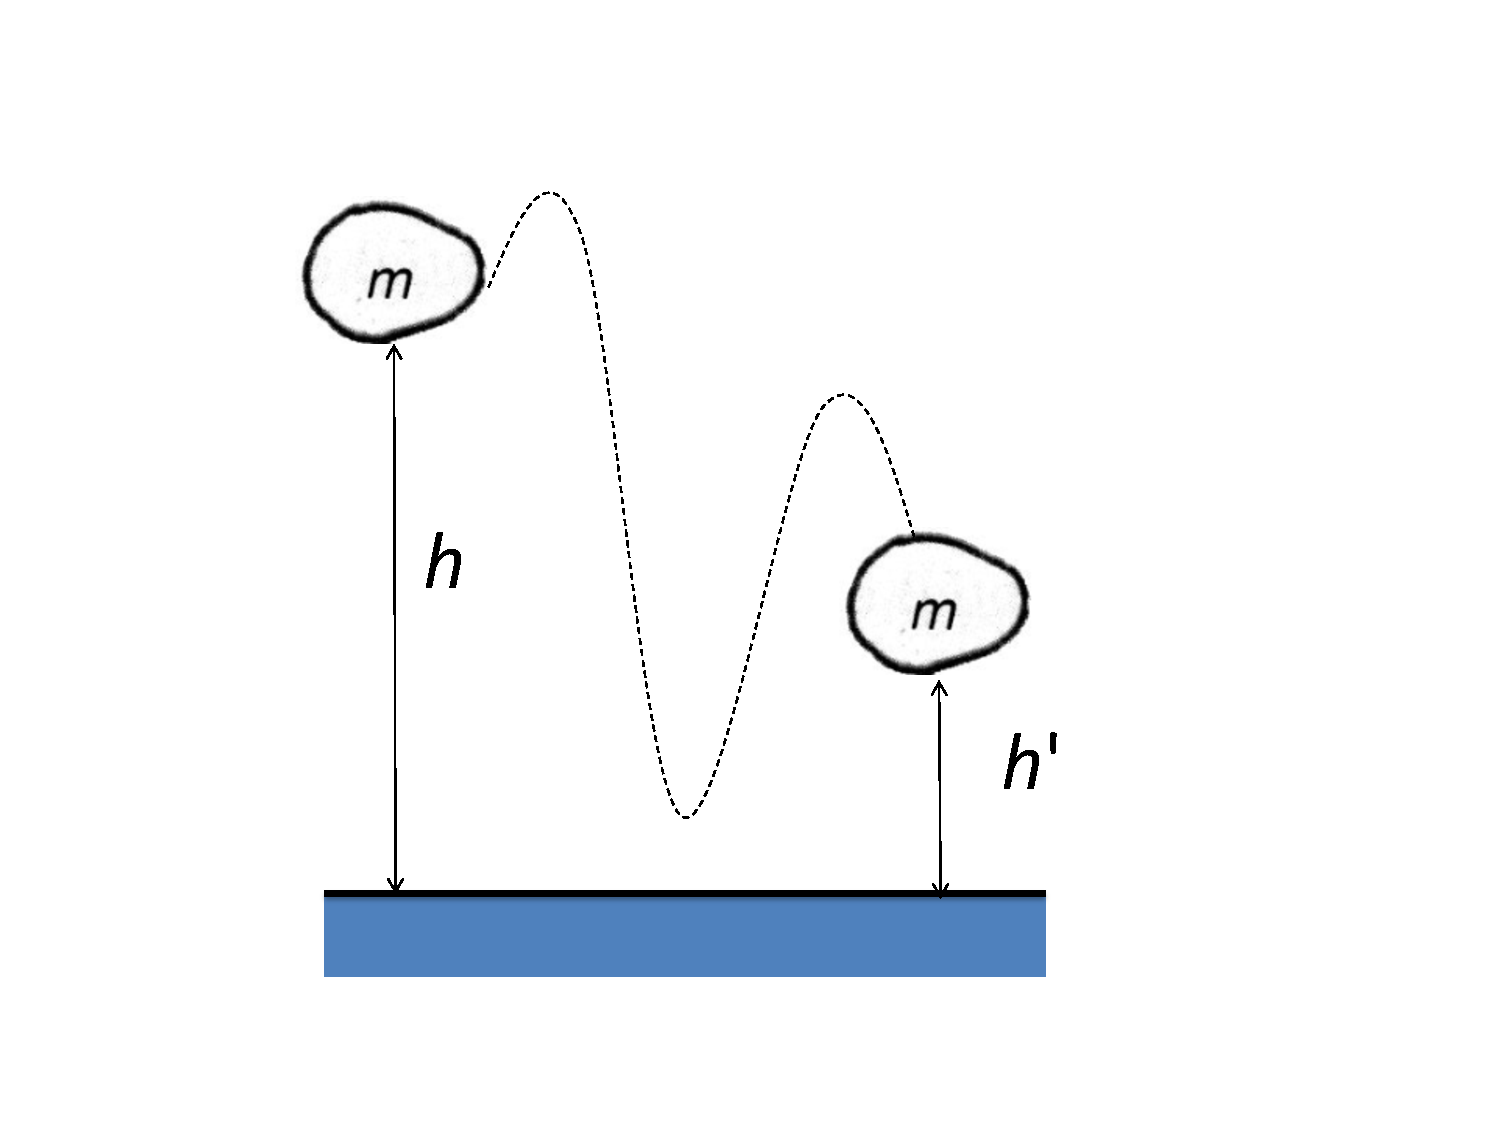
\includegraphics[scale=0.5]{img/potential-energy}
  \caption{重力势能}
  \label{fig:potential-energy}
\end{figure}

图\ref{fig:potential-energy}描述了这一概念。

我们用同样的方法来考虑斐波那契堆的弹出操作,为了计算总消耗,我们首先定义删除最小元素前的势为$\Phi(H)$。这个势是由迄今为止的插入和合并操作累积的。经过树的归并操作,我们得到了新的堆$H'$,由此计算新的势$\Phi(H')$。两个势$\Phi(H')$和$\Phi(H)$的差再加上树归并算法消耗的部分就可以给出弹出操作的分摊复杂度。

为了分析弹出操作,定义势为:

\be
\Phi(H) = t(H)
\ee

其中$t(H)$是斐波那契堆森林中树的棵数。对于任何非空的堆,我们有$t(H) = 1 + length(\mathbb{T})$。

对于$n$个节点的斐波那契堆,设所有树的Rank上限为$D(n)$。经过归并,保证堆森林中树的棵数最多为$D(n)+1$。

在归并前,我们还做了另外一个重要的操作,也对总运行时间有所贡献:我们将存有最小元素的树根删除,然后将其全部子树添加到森林中。因此树归并操作最多处理$D(n) + t(H) - 1$棵树。

总结上述各个因素,我们可以推导出分摊性能如下:

\be
\begin{array}{lll}
T & = & T_{consolidation} + \Phi(H') -\Phi(H) \\
  & = & O(D(n)+t(H)-1) + (D(n) + 1) - t(H) \\
  & = & O(D(n))
\end{array}
\ee

如果只执行过插入、合并和弹出操作,可以确保斐波那契堆中的所有树都为二项式树。因此可以很容易地估计出$D(n)$的上限为$O(\lg n)$(考虑极端情况,所有的节点都在唯一的一棵二项式树中)。

但是,接下来的一节中我们会介绍,存在一种操作会破坏树为二项式树的约定。

\begin{Exercise}
为何树归并操作的时间和它处理的树的数目成比例?
\end{Exercise}

\subsection{减小key}
\index{斐波那契堆!减小key}

还有一种特殊的堆操作,它只在命令式的环境下存在。这个操作就是将某个节点的值减小。减小节点的值对于某些图算法,例如最小生成树算法和Dijkstra算法非常重要\cite{CLRS},而且我们需要这一操作的分摊性能达到常数时间$O(1)$。

但是我们无法定义一个高效的函数$Decrease(H, k, k')$,使得它先定位到key等于$k$的节点,然后将$k$替换为$k'$,最后再恢复堆性质。这是由于如果没有指向目标节点的引用,定位一个节点的时间为$O(n)$。

在命令式的环境中,我们可以定义算法\textproc{Decrease-Key}($H, x, k$)。其中$x$是堆$H$中一个节点的引用,我们希望将它的值减小到$k$。使用$x$,我们无需再执行查找操作,因此有可能给出分摊复杂度为常数时间$O(1)$的算法。

\begin{figure}[htbp]
  \centering
  \setlength{\unitlength}{1cm}
  \begin{picture}(12, 7)
    \put(0, 0){\includegraphics[scale=0.7]{img/cut-fib-tree}}
    \put(6.7, 3){\line(1, 1){0.5}}
    \put(6.7, 3.5){\line(1, -1){0.5}}
  \end{picture}
  \caption{$x<y$,将子树$x$从其父节点上切下,然后添加到森林中。} \label{fig:cut-fib-tree}
\end{figure}

图\ref{fig:cut-fib-tree}描述了这一情况。将节点$x$的值减小后,它小于$y$,我们将$x$从其父节点$y$切下,然后将根为$x$的树“粘贴”到森林中。

虽然我们恢复了堆性质使得父节点的值小于所有的子树,但是由于切除了某些子树,它不再是一棵二项式树了。如果一棵树被切除了很多子树,就无法保证合并操作的性能了。为了避免这一问题,斐波那契堆增加了另外一个限制条件:

“如果一个节点失去了它的第二个子节点,它被立即从父节点切下,然后添加到森林中。”

最终的\textproc{Decrease-Key}算法实现如下:

\begin{algorithmic}[1]
\Function{Decrease-Key}{$H, x, k$}
  \State \Call{Key}{$x$} $\gets k$
  \State $p \gets $ \Call{Parent}{$x$}
  \If{$p \neq NIL \land k < $ \Call{Key}{$p$}}
    \State \Call{Cut}{$H, x$}
    \State \Call{Cascading-Cut}{$H, p$}
  \EndIf
  \If{$k <$ \Call{Key}{$T_{min}(H)$}}
    \State $T_{min}(H) \gets x$
  \EndIf
\EndFunction
\end{algorithmic}

其中函数\textproc{Cascading-Cut}使用一个标记来记录它是否失去第二个子节点。当节点失去第一个子节点时被加上这个标记。在函数\textproc{Cut}中清除这一标记。

\begin{algorithmic}[1]
\Function{Cut}{$H, x$}
  \State $p \gets $ \Call{Parent}{$x$}
  \State remove $x$ from $p$
  \State \Call{Degree}{$p$} $\gets$ \Call{Degree}{$p$} - 1
  \State add $x$ to root list of $H$
  \State \Call{Parent}{$x$} $\gets NIL$
  \State \Call{Mark}{$x$} $\gets FALSE$
\EndFunction
\end{algorithmic}

在级联切除(cascading cut)过程中,若节点$x$被标记了,说明它已经失去了一个子节点。我们递归对其父节点执行切除和级联切除直到达到根节点。

\begin{algorithmic}[1]
\Function{Cascading-Cut}{$H, x$}
  \State $p \gets $ \Call{Parent}{$x$}
  \If{$p \neq NIL$}
    \If{\Call{Mark}{$x$} $= FALSE$}
      \State \Call{Mark}{$x$} $\gets TRUE$
    \Else
      \State \Call{Cut}{$H, x$}
      \State \Call{Cascading-Cut}{$H, p$}
    \EndIf
  \EndIf
\EndFunction
\end{algorithmic}

下面的C语言例子程序实现了减小key的算法。

\lstset{language=C}
\begin{lstlisting}
void decrease_key(struct FibHeap* h, struct node* x, Key k) {
    struct node* p = x->parent;
    x->key = k;
    if(p && k < p->key) {
        cut(h, x);
        cascading_cut(h, p);
    }
    if(k < h->minTr->key)
        h->minTr = x;
}

void cut(struct FibHeap* h, struct node* x) {
    struct node* p = x->parent;
    p->children = remove_node(p->children, x);
    p->degree--;
    h->roots = append(h->roots, x);
    x->parent = NULL;
    x->mark = 0;
}

void cascading_cut(struct FibHeap* h, struct node* x) {
    struct node* p = x->parent;
    if(p) {
        if(!x->mark)
            x->mark = 1;
        else {
            cut(h, x);
            cascading_cut(h, p);
        }
    }
}
\end{lstlisting}

\begin{Exercise}
证明\textproc{Decrease-Key}算法的分摊复杂度为常数时间$O(1)$。
\end{Exercise}

\subsection{斐波那契堆名字的由来}

最后,我们来解释为什么这个数据结构的名字叫作“斐波那契堆”。

我们还剩下一个算法没有给出实现―\textproc{Max-Degree}($n$)。它用来给出含有$n$个节点的斐波那契堆中任意节点degree的上限。我们将用斐波那契数列的性质来给出证明,并最终实现\textproc{Max-Degree}算法。

\begin{lemma}
\label{lemma:Fib-degree}
堆斐波那契堆中的任何节点$x$,记$k = degree(x)$,$|x| = size(x)$,存在以下关系:

\be
  |x| \geq F_{k+2}
\ee

其中$F_k$为斐波那契数列:

\[
F_k = \left \{
  \begin{array}
  {r@{\quad:\quad}l}
  0 & k = 0 \\
  1 & k = 1 \\
  F_{k-1} + F_{k-2} & k \geq 2
  \end{array}
\right.
\]
\end{lemma}

\begin{proof}[证明]
考虑节点$x$的全部$k$棵子树,将它们记为:$y_1, y_2, ..., y_k$,顺序按照它们被链接到$x$时间的先后。其中$y_1$是最早被加入的,而$y_k$是最新加入的。

显然有$|y_i| \geq 0$。当$y_i$链接到$x$的时候,子树$y_1, y_2, ..., y_{i-1}$已经存在了。因为算法只会把Rank相同的树链接起来,所以在这一时刻,我们有:

\[
  degree(y_i) = degree(x) = i - 1
\]

此后,节点$y_i$最多只能失去一个子节点(通过减小key操作),否则一旦失去第二个子节点,它会被立即切除并加入到森林中。因此我们可以推断,对任何$i = 2, 3, ..., k$,有:

\[
degree(y_i) \geq i-2
\]

令$s_k$为节点$x$含有子节点个数\underline{可能的最小值},其中$degree(x) = k$。对于边界情况,有$s_0 = 1$, $s_1 = 2$,对于其他情况,可以推出:

\bea*{rcl}
|x| & \geq & s_k \\
    & =   & 2 + \sum_{i=2}^{k} s_{degree(y_i)} \qquad \\
    & \geq & 2 + \sum_{i=2}^{k} s_{i-2}
\eea*

我们接下来要证明$s_k > F_{k+2}$。使用数学归纳法。对于边界情况,我们有$s_0 = 1 \geq F_2 = 1$,以及$s_1 = 2 \geq F_3 = 2$。对于$k \geq 2$的情况,我们有:

\bea*{rcl}
|x| & \geq & s_k \\
    & \geq & 2 + \sum_{i=2}^{k} s_{i-2} \\
    & \geq & 2 + \sum_{i=2}^{k} F_i \\
    & =    & 1 +  \sum_{i=0}^{k} F_i \\
\eea*

现在,我们需要证明

\be
F_{k+2} = 1 +  \sum_{i=0}^{k} F_i
\ee

再次使用数学归纳法:

\begin{itemize}
\item 边界情况:$F_2 = 1 + F_0 = 2$
\item 递归情况:
\bea*{rcl}
  F_{k+2} & = & F_{k+1} + F_k \\
         & = & 1 + \sum_{i=0}^{k-1}F_i + F_k \\
         & = & 1 + \sum_{i=0}^{k} F_i
\eea*
\end{itemize}

综上,我们得到最终结论:
\be
n \geq |x| \geq F_k+2
\ee
\end{proof}

回忆AVL树的结果:$F_k \geq \phi^k$,其中$\phi = \frac{1+\sqrt{5}}{2}$为黄金分割比。我们同时证明了弹出操作的分摊复杂度为$O(\lg n)$。

根据这一结果,我们可以定义函数$MaxDegree$如下:

\be
  MaxDegree(n) = 1 + \lfloor \log_{\phi} n \rfloor
\ee

命令式的\textproc{Max-Degree}算法可以同样使用斐波那契数列来实现:

\begin{algorithmic}[1]
\Function{Max-Degree}{$n$}
  \State $F_0 \gets 0$
  \State $F_1 \gets 1$
  \State $k \gets 2$
  \Repeat
    \State $F_k \gets F_{k_1} + F_{k_2}$
    \State $k \gets k+1$
  \Until{$F_k < n$}
  \State \Return $k-2$
\EndFunction
\end{algorithmic}

下面的C例子程序实现了这一算法:

\lstset{language=C}
\begin{lstlisting}
int max_degree(int n) {
    int k, F;
    int F2 = 0;
    int F1 = 1;
    for(F = F1 + F2, k = 2; F < n; ++k) {
        F2 = F1;
        F1 = F;
        F = F1 + F2;
    }
    return k-2;
}
\end{lstlisting}

% ================================================================
%                 Pairing Heaps
% ================================================================

\section{配对堆}
\label{pairing-heap} \index{配对堆}

虽然斐波那契堆在理论上有着优异的性能,但是它的实现复杂。人们发现斐波那契堆复杂度中big-O后面的常数较大,它的理论意义要大于实际意义。

本节中,我们介绍另外一种堆―配对(pairing)堆。它是已知性能最好的堆。大部分操作,包括插入、获取顶部元素、合并都是常数时间$O(1)$的,人们猜测它的弹出操作的分摊复杂度为$O(\lg n)$\cite{pairing-heap}\cite{okasaki-book}。到作者书写本章为止的15年内,这一猜想还没有得到证明。尽管有大量的试验数据支持它的分摊复杂度为$O(\lg n)$。

除了性能优异,配对堆还很简单。存在简洁的命令式和函数式实现。

% ================================================================
%                 Definition
% ================================================================
\subsection{定义}
\index{配对堆!定义}

二项式堆和斐波那契堆都由森林来实现。而配对堆本质上是一棵$K$叉树。最小元素保存于树根,其余元素存储于子树中。

下面的Haskell程序定义了配对堆。

\lstset{language=Haskell}
\begin{lstlisting}[style=Haskell]
data PHeap a = E | Node a [PHeap a]
\end{lstlisting}

这是一个递归定义,一个配对堆要么为空,要么是一棵$K$叉树,包含一个根节点和一组子树。

下面的C语言例子程序,也给出了配对堆的定义。简单起见,我们仅仅讨论最小堆,并且假设key的类型为整数\footnote{可以将key的类型抽象为C++的模板参数,读者可以参考本书附带的例子程序。}。我们使用单向链表表示的“左侧孩子,右侧兄弟”定义(二叉树表示法\cite{CLRS})。

\lstset{language=C}
\begin{lstlisting}
typedef int Key;

struct node {
    Key key;
    struct node *next, *children, *parent;
};
\end{lstlisting}

其中的父节点字段仅在减小key值的操作中用到,其他情况下可以忽略。我们稍后会加以解释。


% ================================================================
%          Basic Heap operations
% ================================================================
\subsection{基本堆操作}

我们首先介绍堆的合并操作,合并操作可以用以实现插入。获取顶部元素相对简单。而弹出操作则较为复杂。

\subsubsection{合并、插入、和获取顶部元素}
\index{配对堆!插入} \index{配对堆!top}
\index{配对堆!查找最小元素}

合并操作的思想和二项式堆的链接相似。当我们合并两个配对堆时,存在两种情况:

\begin{itemize}
\item 简单情况:其中一个堆为空,我们只要返回另一堆作为合并的结果;

\item 否则,我们比较两个堆的根节点元素,令根节点较大的一个作为另一个的新子树。
\end{itemize}

令$H_1$和$H_2$分别代表两个堆,$x$和$y$为各自的根节点元素。函数$Children()$返回一棵$K$叉树的子树,$Node()$从一个根节点元素和一组子树构造一棵$K$叉树。

\be
merge(H_1, H_2) = \left \{
  \begin{array}
  {r@{\quad:\quad}l}
  H_1 & H_2 = \phi \\
  H_2 & H_1 = \phi \\
  Node(x, \{H_2\} \cup Children(H_1)) & x < y \\
  Node(y, \{H_1\} \cup Children(H_2)) & otherwise
  \end{array}
\right .
\ee

其中

\[
\begin{array}{l}
x = Root(H_1) \\
y = Root(H_2)
\end{array}
\]

显然合并算法的性能为常数时间$O(1)$\footnote{假设$\cup$操作的性能为常数时间。对于单向链表的“cons”来说,这一点成立。}。

下面的Haskell例子程序给出了$merge$操作。

\lstset{language=Haskell}
\begin{lstlisting}[style=Haskell]
merge h E = h
merge E h = h
merge h1@(Node x hs1) h2@(Node y hs2) =
    if x < y then Node x (h2:hs1) else Node y (h1:hs2)
\end{lstlisting}

也可以用命令式的方式实现合并操作。使用“左侧孩子,右侧兄弟”方法,我们可以把根节点元素较大的堆,利用链表操作链接到另一个堆的子树前面变成第一棵子树。这一常数时间的操作可以描述如下:

\begin{algorithmic}[1]
\Function{Merge}{$H_1, H_2$}
  \If{$H_1 = $ NIL}
    \State \Return $H_2$
  \EndIf
  \If{$H_2 = $ NIL}
    \State \Return $H_1$
  \EndIf
  \If{\Call{Key}{$H_2$} $<$ \Call{Key}{$H_1$}}
    \State \Call{Exchange}{$H_1 \leftrightarrow H_2$}
  \EndIf
  \State Insert $H_2$ in front of \Call{Children}{$H_1$}
  \State \Call{Parent}{$H_2$} $\gets H_1$
  \State \Return $H_1$
\EndFunction
\end{algorithmic}

在这一过程中,我们也更新了指向父节点的字段。相应的C语言例子代码如下:

\lstset{language=C}
\begin{lstlisting}
struct node* merge(struct node* h1, struct node* h2) {
    if (h1 == NULL)
        return h2;
    if (h2 == NULL)
        return h1;
    if (h2->key < h1->key)
        swap(&h1, &h2);
    h2->next = h1->children;
    h1->children = h2;
    h2->parent = h1;
    h1->next = NULL; /*Break previous link if any*/
    return h1;
}
\end{lstlisting}

其中swap函数和斐波那契堆中的定义类似。

使用合并函数,可以像斐波那契堆的式(\ref{eq:fib-insert})一样实现插入操作。这一操作的性能为常数时间$O(1)$。因为最小的元素总是保存在根节点,所以可以通过根来获取顶部元素。

\be
top(H) = Root(H)
\ee

获取顶部元素的性能也是常数时间$O(1)$的。

\subsubsection{减小节点的值}
\index{配对堆!减小key}

同斐波那契堆一样,减小节点的值仅在命令式环境下有意义。这一问题的解比斐波那契堆要简单。节点的值减小后,我们将它为根的子树从父节点上切下,然后合并到堆中。唯一特殊的情况是,如果是根节点,我们可以直接改变值而无需做任何额外操作。

下面的算法描述了将节点$x$的值减小到$k$的操作。

\begin{algorithmic}[1]
\Function{Decrease-Key}{$H, x, k$}
  \State \Call{Key}{$x$} $\gets k$
  \If{\Call{Parent}{$x$} $\neq$ NIL}
    \State Remove $x$ from \textproc{Children}(\Call{Parent}{$x$})
    \Call{Parent}{$x$} $\gets$ NIL
    \State \Return \Call{Merge}{$H, x$}
  \EndIf
  \State \Return $H$
\EndFunction
\end{algorithmic}

下面的C语言例子程序实现了这一算法。

\lstset{language=C}
\begin{lstlisting}
struct node* decrease_key(struct node* h, struct node* x, Key key) {
    x->key = key; /* Assume key <= x->key */
    if(x->parent) {
        x->parent->children = remove_node(x->parent->children, x);
        x->parent = NULL;
        return merge(h, x);
    }
    return h;
}
\end{lstlisting}

\begin{Exercise}
选择一门语言,实现从父节点将子树切下的操作。考虑如何保证减小key操作的总体性能为常数时间$O(1)$?仅仅使用“左侧孩子,右侧兄弟”就够了么?
\end{Exercise}

\subsubsection{弹出}
\index{配对堆!pop} \index{配对堆!弹出}
\index{配对堆!删除最小元素}

因为最小元素总是保存在根节点,弹出操作将其删除后,会剩下一系列子树。这些子树可以合并成一棵较大的树。

\be
  pop(H) = mergePairs(Children(H))
\ee

配对堆使用一种特殊的合并策略,它先从左向右,两两成对地将子树合并。然后从右向左将子树对合并的结果再次合并成一棵树。配对堆的名字就来自这一合并过程。

图\ref{fig:merge-pairs}和\ref{fig:merge-right}描述了这一成对合并的过程。

\begin{figure}[htbp]
  \centering
  \subcaptionbox{弹出前的配对堆}{\includegraphics[scale=0.5]{img/pairing-hp}} \\
  \subcaptionbox{根节点2被删除,剩余9棵子树}{\includegraphics[scale=0.5]{img/pairs}} \\
  \subcaptionbox{每两棵树成对合并,因为有奇数棵树,所以最后一棵无需合并。}{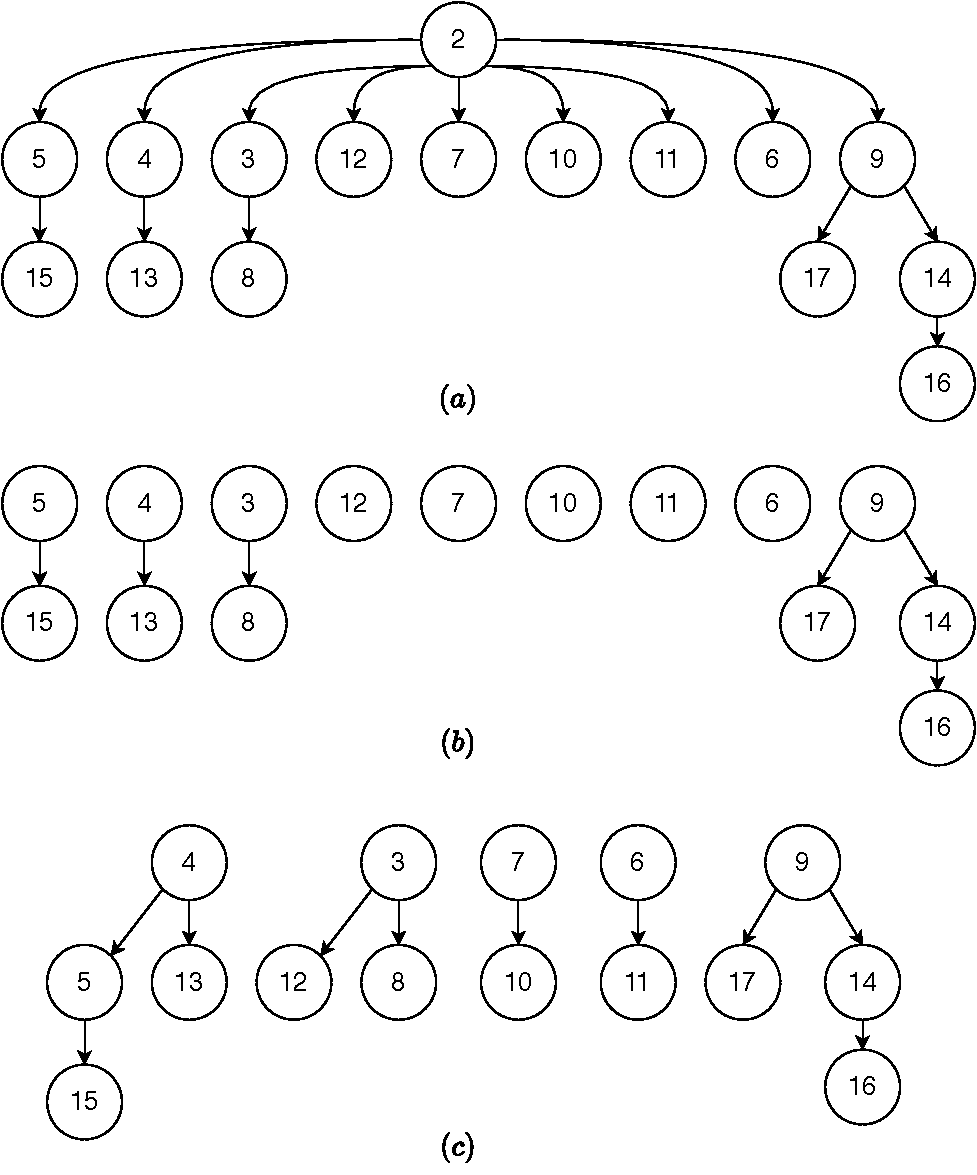
\includegraphics[scale=0.5]{img/pairs-merge}} \\
  \caption{删除根节点,将子树成对合并} \label{fig:merge-pairs}
\end{figure}

\begin{figure}[htbp]
  \centering
  \subcaptionbox{将根节点为9和6的两棵树合并}{\hspace{0.2\textwidth}\includegraphics[scale=0.5]{img/right-merge-1}\hspace{0.2\textwidth}}
  \subcaptionbox{将根节点为7的树合并到当前结果中}{\hspace{0.1\textwidth}\includegraphics[scale=0.5]{img/right-merge-2}\hspace{0.1\textwidth}} \\
  \subcaptionbox{将根节点为3的树合并到结果中}{\hspace{0.1\textwidth}\includegraphics[scale=0.5]{img/right-merge-3}\hspace{0.1\textwidth}}
  \subcaptionbox{将根节点为4的树合并到结果中}{\hspace{0.1\textwidth}\includegraphics[scale=0.5]{img/right-merge-4}\hspace{0.1\textwidth}}
  \caption{从右向左合并的步骤} \label{fig:merge-right}
\end{figure}

递归地成对合并过程和自底向上的归并排序\cite{okasaki-book}类似。记配对堆的全部子树为$A$,它是一个子树的列表$\{ T_1, T_2, T_3, ..., T_m\}$。$mergePairs()$函数定义如下:

\be
mergePairs(A) = \left \{
  \begin{array}
  {r@{\quad:\quad}l}
  \Phi & A = \Phi \\
  T_1 & A = \{ T_1 \} \\
  merge(merge(T_1, T_2), mergePairs(A')) & otherwise
  \end{array}
\right .
\ee

其中

\[
A' = \{ T_3, T_4, ..., T_m\}
\]

是除去前两棵树外剩余的子树。

下面的Haskell例子程序实现了这一算法。

\lstset{language=Haskell}
\begin{lstlisting}[style=Haskell]
deleteMin (Node _ hs) = mergePairs hs where
    mergePairs [] = E
    mergePairs [h] = h
    mergePairs (h1:h2:hs) = merge (merge h1 h2) (mergePairs hs)
\end{lstlisting}

弹出操作也可以按照过程描述如下:

\begin{algorithmic}[1]
\Function{Pop}{$H$}
  \State $L \gets NIL$
  \For{every 2 trees $T_x$, $T_y \in$ \Call{Children}{$H$} from left to right}
    \State Extract $x$, and $y$ from \Call{Children}{$H$}
    \State $T \gets $ \Call{Merge}{$T_x, T_y$}
    \State Insert $T$ at the beginning of $L$
  \EndFor
  \State $H \gets $ \Call{Children}{$H$} \Comment{$H$ is either $NIL$ or one tree.}
  \For{$\forall T \in L$ from left to right}
    \State $H \gets $ \Call{Merge}{$H, T$}
  \EndFor
  \State \Return $H$
\EndFunction
\end{algorithmic}

其中$L$被初始化为一个空的链表,然后算法从左向右每次成对迭代$K$叉树中的两棵子树,进行合并。结果被插入到$L$的头部。因为在链表的前方插入,所以再次遍历链表$L$时,实际是按照从右向左的顺序。堆$H$中可能含有奇数棵子树,这种情况下,成对合并后会剩余一棵。处理办法是从这一棵树开始进行从右向左的合并。

下面的C语言例子程序实现了弹出算法。

\lstset{language=C}
\begin{lstlisting}
struct node* pop(struct node* h) {
    struct node *x, *y, *lst = NULL;
    while ((x = h->children) != NULL) {
        if ((h->children = y = x->next) != NULL)
            h->children = h->children->next;
        lst = push_front(lst, merge(x, y));
    }
    x = NULL;
    while((y = lst) != NULL) {
        lst = lst->next;
        x = merge(x, y);
    }
    free(h);
    return x;
}
\end{lstlisting}

人们猜想配对堆的弹出操作的分摊性能为$O(\lg n)$\cite{pairing-heap}。

\begin{Exercise}
选择一门语言,实现在链表的头部插入一棵树。
\end{Exercise}

\subsubsection{删除节点}
\index{配对堆!删除}

我们没有在二项式堆和斐波那契堆提到删除操作。删除可以实现为先将节点的值减小为负无穷($-\infty$),然后再执行一次弹出操作。这里我们介绍另外一种删除方法。

我们需要定义函数$delete(H, x)$,其中$x$是配对堆$H$中的某一节点\footnote{具体来说,$x$是某一节点的引用}。

若$x$为根节点,我们只需要执行一次弹出操作。否则,我们将$x$从$H$中切下,然后对$x$执行一次弹出操作,再将弹出结果合并回$H$。如下:

\be
delete(H, x) = \left \{
  \begin{array}
  {r@{\quad:\quad}l}
  pop(H) & x \quad \text{is root of} \quad H \\
  merge(cut(H, x), pop(x)) & otherwise
  \end{array}
\right .
\ee

因为删除算法调用弹出操作,因此人们猜想它的分摊性能也是对数时间$O(\lg n)$。

\begin{Exercise}
\begin{itemize}
\item 选择一门语言,实现命令式的删除算法。

\item 考虑如何完整实现纯函数式的删除算法。
\end{itemize}
\end{Exercise}

% ================================================================
%                 Short summary
% ================================================================
\section{小结}

本章中,我们将堆的实现从二叉树扩展到了更加丰富的数据结构。二项式堆和斐波那契堆使用$K$叉树的森林作为底层数据结构,而配对堆使用一棵$K$叉树来存储数据。通过将某些费时的操作延迟进行,可以获得总体上优异的分摊性能。这一点很具有启发性。虽然斐波那契堆在理论上具有良好的性能,但是实现较为复杂,最近的一些教科书往往会跳过不讲。本章介绍的配对堆具备简单的实现,并且在实际应用中性能表现很好。

到本章为止,我们介绍了一些最基本的基于树的数据结构。还有大量和树有关的内容有待我们去了解和探索。从下一章开始,我们将介绍通用的序列数据结构,包括数组和队列。

\section{附录:例子程序}

多叉树的定义(左侧孩子,右侧兄弟):

\begin{lstlisting}[language = Bourbaki]
data Node<K> {
    Int rank
    K key
    Node<K> parent
    Node<K> subTrees
    Node<K> sibling

    Node(K x) {
        key = x
        rank = 0
        parent = subTrees = sibling = null
    }
}
\end{lstlisting}

二项式树链接:

\begin{lstlisting}[language = Bourbaki]
Node<K> link(Node<K> t1, Node<K> t2) {
    if t2.key < t1.key then (t1, t2) = (t2, t1)
    t2.sibling = t1.subTrees
    t1.subTrees = t2
    t2.parent = t1
    t1.rank = t1.rank + 1
    return t1
}
\end{lstlisting}

二项式堆插入:

\begin{lstlisting}[language = Bourbaki]
Node<K> insertTree(Node<K> t, Node<K> h) {
    var h1 = Node()
    var prev = h1
    while h != null and h.rank <= t.rank {
        var t1 = h
        h = h.sibling
        if t.rank == t1.rank {
            t = link(t, t1)
        } else {
            prev.sibling = t1
            prev = t1
        }
    }
    prev.sibling = t
    t.sibling = h
    return removeFirst(h1)
}

Node<K> removeFirst(Node<K> h) {
    var next = h.sibling
    h.sibling = null
    return next
}

Node<K> insert(K x, Node<K> h) = insertTree(Node(x), h)
\end{lstlisting}

二项式堆的合并:

\begin{lstlisting}[language = Bourbaki]
Node<K> merge(h1, h2) {
    var h = Node()
    var prev = h
    while h1 != null and h2 != null {
        if h1.rank < h2.rank {
            prev.sibling = h1
            prev = prev.sibling
            h1 = h1.sibling
        } else if h2.rank < h1.rank {
            prev.sibling = h2
            prev = prev.sibling
            h2 = h2.sibling
        } else {
            var (t1, t2) = (h1, h2)
            (h1, h2) = (h1.sibling, h2.sibling)
            h1 = insertTree(link(t1, t2), h1)
    }
    if h1 != null then prev.sibling = h1
    if h2 != null then prev.sibling = h2
    return removeFirst(h)
}
\end{lstlisting}

二项式堆的弹出

\begin{lstlisting}[language = Bourbaki]
Node<K> reverse(Node<K> h) {
    Node<K> prev = null
    while h != null {
        var x = h
        h = h.sibling
        x.sibling = prev
        prev = x
    }
    return prev
}

(Node<K>, Node<K>) extractMin(Node<K> h) {
    var head = h
    Node<K> tp = null
    Node<K> tm = null
    Node<K> prev = null
    while h != null {
        if tm == null or h.key < tm.key {
            tm = h
            tp = prev
        }
        prev = h
        h = h.sibling
    }
    if tp != null {
        tp.sibling = tm.sibling
    } else {
        head = tm.sibling
    }
    tm.sibling = null
    return (tm, head)
}

(K, Node<K>) pop(Node<K> h) {
    var (tm, h) = extractMin(h)
    h = merge(h, reverse(tm.subtrees))
    tm.subtrees = null
    return (tm.key, h)
}
\end{lstlisting}

\ifx\wholebook\relax \else
\section{参考答案}
\shipoutAnswer

\begin{thebibliography}{99}

\bibitem{K-ary-tree}
K-ary tree, Wikipedia. \url{https://en.wikipedia.org/wiki/K-ary_tree}

\bibitem{CLRS}
Thomas H. Cormen, Charles E. Leiserson, Ronald L. Rivest and Clifford Stein. ``Introduction to Algorithms, Second Edition''. The MIT Press, 2001. ISBN: 0262032937. (《算法导论》中文版)

\bibitem{okasaki-book}
Chris Okasaki. ``Purely Functional Data Structures''. Cambridge university press, (July 1, 1999), ISBN-13: 978-0521663502

\bibitem{wiki-pascal-triangle}
Wikipedia, ``Pascal's triangle''. \url{https://en.wikipedia.org/wiki/Pascal's_triangle}

\bibitem{hackage-fibq}
Hackage. ``An alternate implementation of a priority queue based on a Fibonacci heap.'', \url{http://hackage.haskell.org/packages/archive/pqueue-mtl/1.0.7/doc/html/src/Data-Queue-FibQueue.html}

\bibitem{okasaki-fibh}
Chris Okasaki. ``Fibonacci Heaps.'' \url{http://darcs.haskell.org/nofib/gc/fibheaps/orig}

\bibitem{pairing-heap}
Michael L. Fredman, Robert Sedgewick, Daniel D. Sleator, and Robert E. Tarjan. ``The Pairing Heap: A New Form of Self-Adjusting Heap'' Algorithmica (1986) 1: 111-129.

\end{thebibliography}

\expandafter\enddocument
\fi
